% Created 2019-09-05 jue 12:34
\documentclass[letterpaper]{scrartcl}
\usepackage[utf8]{inputenc}
\usepackage[T1]{fontenc}
\usepackage{fixltx2e}
\usepackage{graphicx}
\usepackage{longtable}
\usepackage{float}
\usepackage{wrapfig}
\usepackage{rotating}
\usepackage[normalem]{ulem}
\usepackage{amsmath}
\usepackage{textcomp}
\usepackage{marvosym}
\usepackage{wasysym}
\usepackage{amssymb}
\usepackage{hyperref}
\tolerance=1000
\usepackage{khpreamble}
\usepackage{subfigure}
\usepgfplotslibrary{groupplots}
\addtolength{\oddsidemargin}{-4mm}
\addtolength{\evensidemargin}{-4mm}
\addtolength{\textheight}{33mm}
\author{Kjartan Halvorsen}
\date{}
\title{}
\hypersetup{
  pdfkeywords={},
  pdfsubject={},
  pdfcreator={Emacs 25.3.50.2 (Org mode 8.2.10)}}
\begin{document}



\section*{Root locus, Bode- and Nyquist plots, relative stability}
\label{sec-1}
Kjartan Halvorsen, September 2019

\subsection*{Draw a root locus for PI-control of the reservoir}
\label{sec-1-1}
\begin{center}
  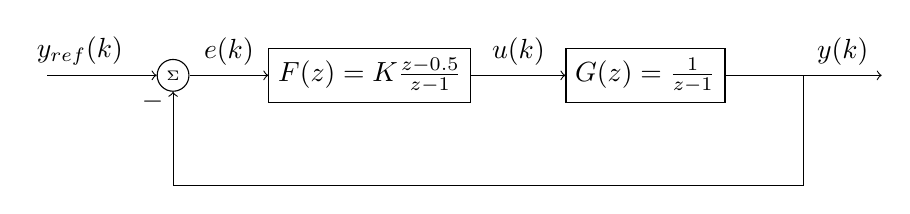
\begin{tikzpicture}[node distance=22mm, block/.style={rectangle, draw, minimum width=15mm}, sumnode/.style={circle, draw, inner sep=2pt}]
    
    \node[coordinate] (input) {};
    \node[sumnode, right of=input, node distance=16mm] (sum) {\tiny $\Sigma$};
    \node[block, right of=sum, node distance=25mm] (controller)  {$F(z) = K\frac{z-0.5}{z-1}$};
    \node[block, right of=controller, node distance=35mm] (plant)  {$G(z) = \frac{1}{z-1}$};
    \node[coordinate, right of=plant, node distance=30mm] (output) {};

    \draw[->] (input) -- node[above, pos=0.3] {$y_{ref}(k)$} (sum);
    \draw[->] (sum) -- node[above] {$e(k)$} (controller);
    \draw[->] (controller) -- node[above] {$u(k)$} (plant);
    \draw[->] (plant) -- node[coordinate] (measure) {}  node[above, near end] {$y(k)$} (output);
    \draw[->] (measure) -- ++(0,-14mm) -| node[pos=0.95, left] {$-$} (sum);
  \end{tikzpicture}
\end{center}

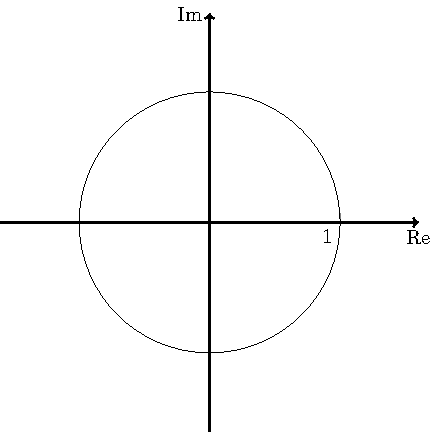
\includegraphics[width=0.36\linewidth]{../../figures/imaginary-plane-empty}
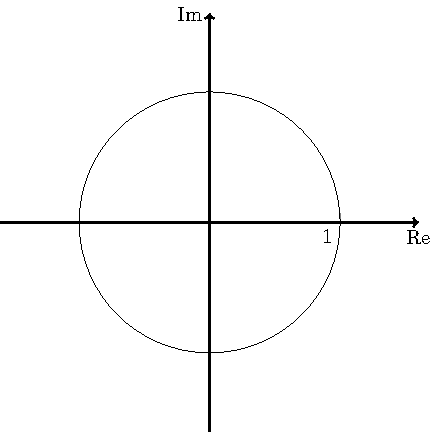
\includegraphics[width=0.36\linewidth]{../../figures/imaginary-plane-empty}\\

\subsection*{Frequency response primer: The product of two complex numbers}
\label{sec-1-2}
\begin{itemize}
\item At time \(k=2\), the discrete-time complex exponential signal \(u(k) = \mathrm{e}^{i\frac{\pi}{12}k}\) has the value \(u(2) = \mathrm{e}^{i\frac{\pi}{6}}\).
\item A pulse-transfer function \(H(z)\) is a mapping from the complex plane to the complex plane, that is \( H: \; \mathbb{C} \rightarrow \mathbb{C}\). Consider a specific pulse-transfer function \(H(z)\) that when evaluated at \(z=\mathrm{e}^{i\frac{\pi}{12}}\) has the value  \(H(\mathrm{e}^{i\frac{\pi}{12}}) = 2\mathrm{e}^{-i\frac{\pi}{3}}\).
\end{itemize}

\textbf{Determine the magnitude, the argument and the imaginary part of the product \(H(\mathrm{e}^{i\frac{\pi}{12}})u(2)\). Then mark the first few values of the sequence \(H(\mathrm{e}^{i\frac{\pi}{12}})u(k)\).}

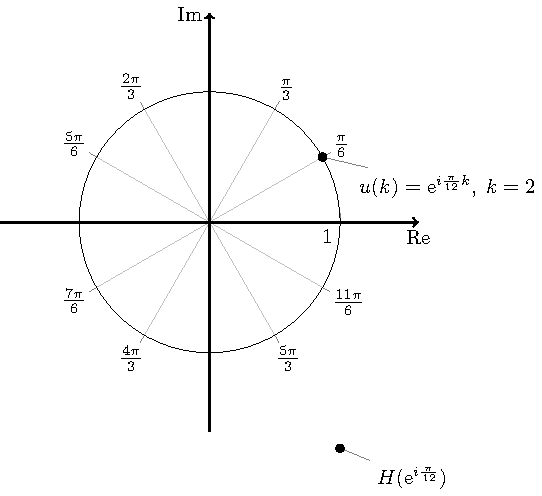
\includegraphics[width=0.34\linewidth]{../../figures/imaginary-plane-two-points}


\subsection*{Bode plot and Nyquist plots}
\label{sec-1-3}
Sketch the Nyquist plot corresponding to the Bode plot! Then mark the phase margin and amplitude margins!
\begin{center}
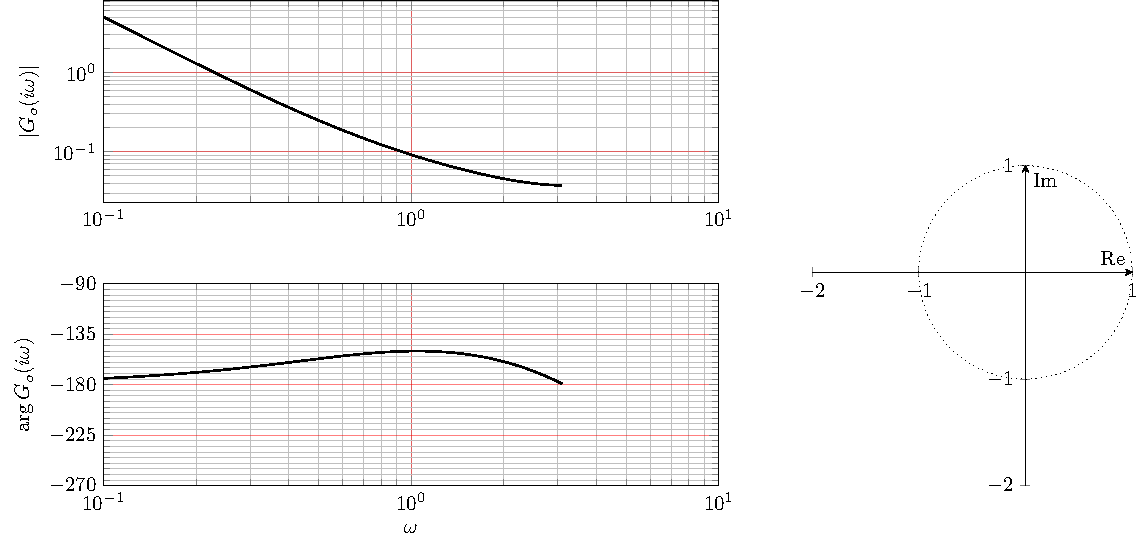
\includegraphics[width=0.95\linewidth]{../../figures/bode-nyquist-exc-1}
\end{center}

\begin{center}
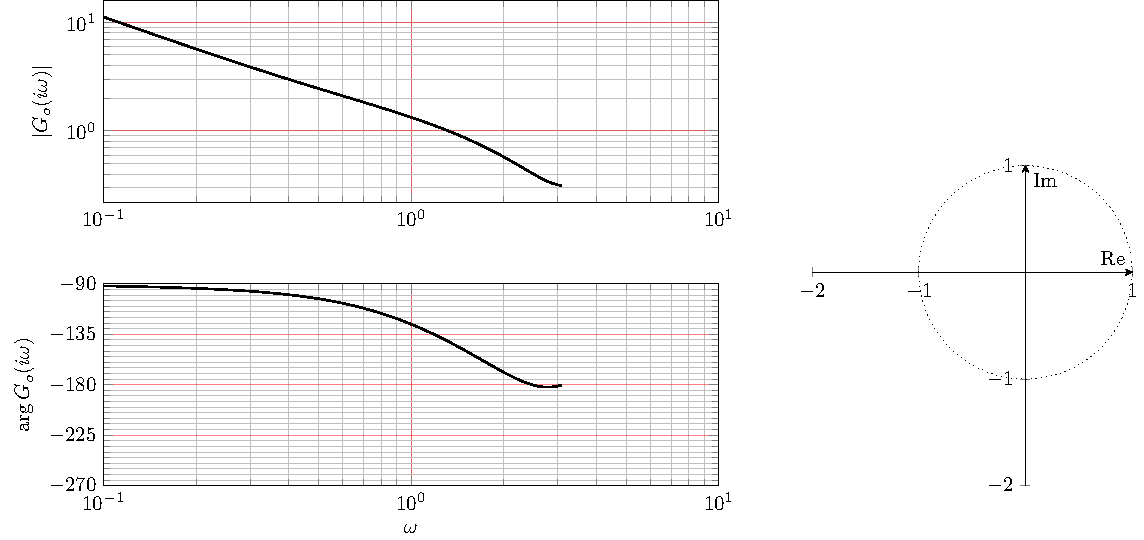
\includegraphics[width=0.95\linewidth]{../../figures/bode-nyquist-exc-2}
\end{center}
% Emacs 25.3.50.2 (Org mode 8.2.10)
\end{document}